\chapter{Ions and Ionic Solutions}\label{ch:g9:ions}

Two clear drinks stand on a gym bench: a bottle of sports drink, sold for
its ``electrolytes'', and a glass of sugared water. In a laboratory, two
metal plates connected to a battery and a small bulb are dipped into
each in turn. In the sports drink the bulb lights up; in the sugared
water it stays dark. Something in the first liquid carries electric
charge, and the sugar does not. That something is \omterm{def:g9:ions:ion}{ions}.

\begin{recall}
An \omterm{def:g7:atoms-and-molecules:atom}{atom} has a \omterm{def:g9:inside-the-atom:nucleus}{nucleus} with $Z$ \omterm{def:g9:inside-the-atom:proton}{protons}, each of charge $+e$, and $Z$
\omterm{def:g9:inside-the-atom:nucleus}{electrons} around it, each of charge $-e$: the \omterm{def:g7:atoms-and-molecules:atom}{atom} is neutral
(\cref{ch:g9:inside-the-atom}). A \omterm{def:g6:solutions-and-solubility:solute}{solute} dissolved in water gives an
\omterm{def:g6:solutions-and-solubility:solute}{aqueous solution} (\cref{ch:g6:solutions-and-solubility}). A \omterm{def:g7:identifying-substances:characteristic-test}{characteristic
test} detects a species by a visible result
(\cref{ch:g7:identifying-substances}).
\end{recall}

\begin{omfigure}
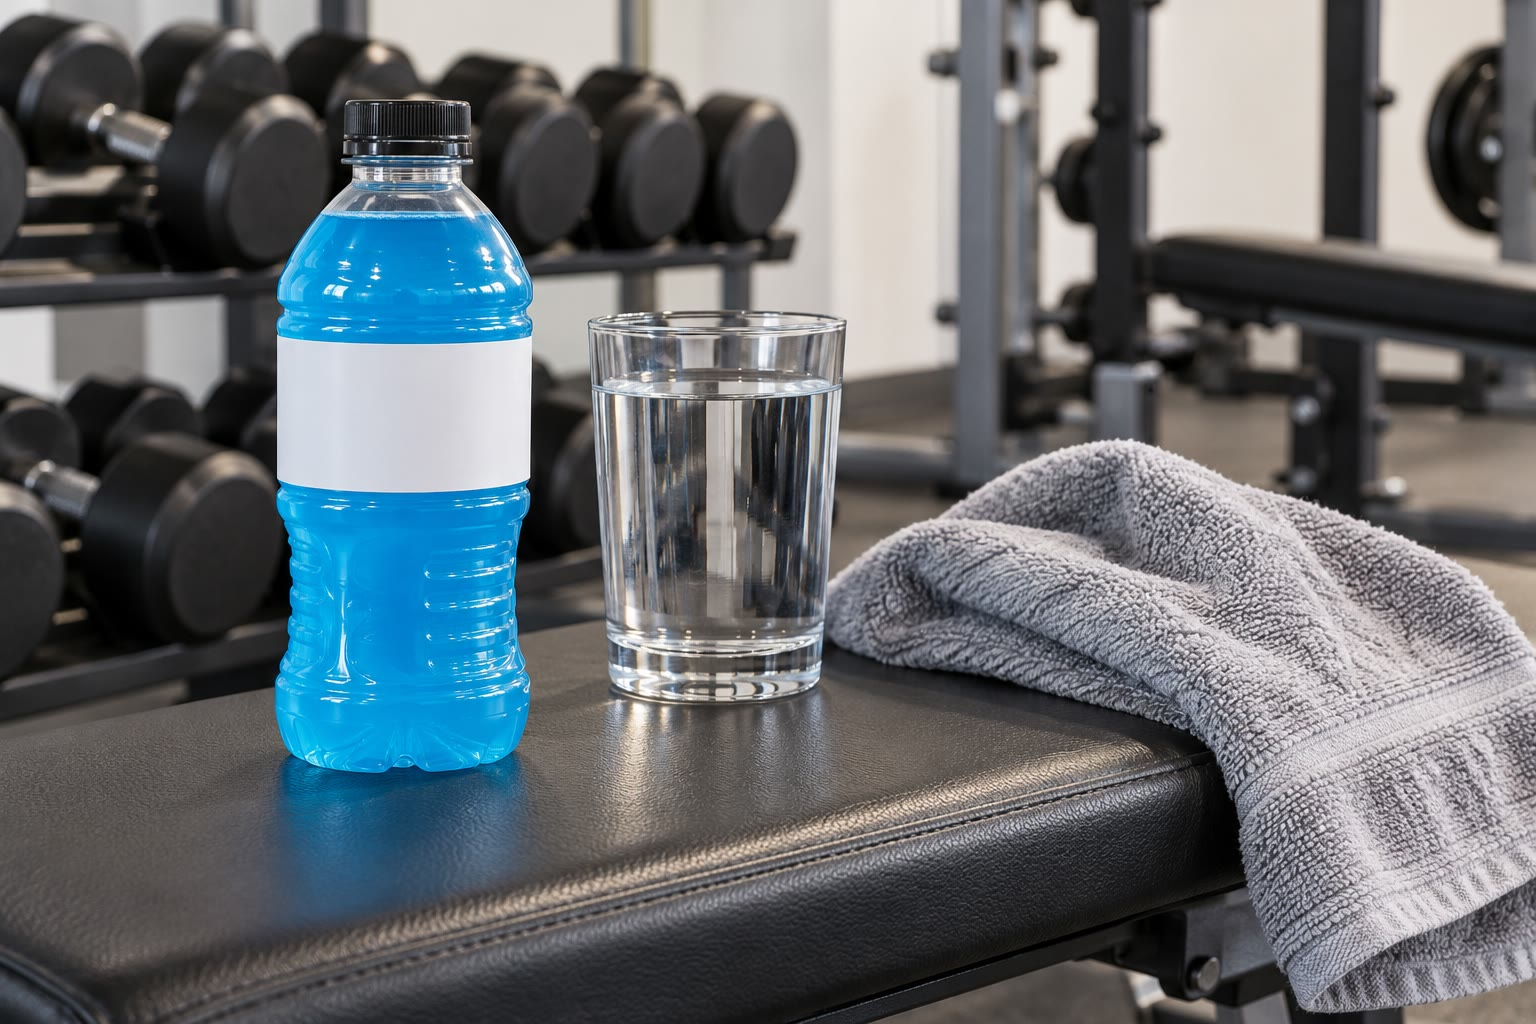
\includegraphics[width=0.5\linewidth]{images/book1/ai/g9-sports-drink.jpg}

{\small A sports drink and a glass of water: the drink contains
dissolved \omterm{def:g9:ions:ion}{ions}.}
\end{omfigure}

\section{Atoms that gain or lose electrons}

\begin{definition}[Ion, cation, anion]\label{def:g9:ions:ion}
An \emph{ion}\index{ion} is an \omterm{def:g7:atoms-and-molecules:atom}{atom}, or a group of \omterm{def:g7:atoms-and-molecules:atom}{atoms}, that has lost or
gained one or more \omterm{def:g9:inside-the-atom:nucleus}{electrons}, and so carries an electric charge. An ion
with a positive charge, having lost \omterm{def:g9:inside-the-atom:nucleus}{electrons}, is a
\emph{cation}\index{cation}; an ion with a negative charge, having gained
\omterm{def:g9:inside-the-atom:nucleus}{electrons}, is an \emph{anion}\index{anion}. The charge is written at the
top right of the formula: \ce{Na+}, \ce{Cu^{2+}}, \ce{Cl-}.
\end{definition}

\begin{example}[Sodium and chlorine]\label{ex:g9:ions:na-cl}
A sodium \omterm{def:g7:atoms-and-molecules:atom}{atom}, 11 \omterm{def:g9:inside-the-atom:proton}{protons} and 11 \omterm{def:g9:inside-the-atom:nucleus}{electrons}, loses one \omterm{def:g9:inside-the-atom:nucleus}{electron}: it
becomes the sodium \omterm{def:g9:ions:ion}{ion} \ce{Na+}, 11 \omterm{def:g9:inside-the-atom:proton}{protons} and 10 \omterm{def:g9:inside-the-atom:nucleus}{electrons}, charge
$+1$:
\[
  \ce{Na -> Na+ + e-}.
\]
A chlorine \omterm{def:g7:atoms-and-molecules:atom}{atom}, 17 \omterm{def:g9:inside-the-atom:proton}{protons} and 17 \omterm{def:g9:inside-the-atom:nucleus}{electrons}, gains one \omterm{def:g9:inside-the-atom:nucleus}{electron}: it
becomes the chloride \omterm{def:g9:ions:ion}{ion} \ce{Cl-}, 17 \omterm{def:g9:inside-the-atom:proton}{protons} and 18 \omterm{def:g9:inside-the-atom:nucleus}{electrons}:
\[
  \ce{Cl + e- -> Cl-}.
\]
\end{example}

\begin{omfigure}
\begin{tikzpicture}[font=\small]
  \foreach \x/\name/\p/\e/\ch/\col in {0/{sodium atom}/11/11/0/omDef,
      3.7/{sodium ion \ce{Na+}}/11/10/+1/omProp,
      8.0/{chlorine atom}/17/17/0/omDef, 11.7/{chloride ion \ce{Cl-}}/17/18/$-1$/omProp} {
    \node[draw=\col, fill=\col!6, rounded corners=2pt, align=center, text width=2.4cm]
      at (\x,0) {\textbf{\name}\\ \p\ protons\\ \e\ electrons\\ charge \ch};
  }
  \draw[->, thick, omProp] (1.45,0) -- (2.25,0) node[midway, above, text=black,
    font=\footnotesize, align=center] {loses\\ 1 \ce{e-}};
  \draw[->, thick, omProp] (9.45,0) -- (10.25,0) node[midway, above, text=black,
    font=\footnotesize, align=center] {gains\\ 1 \ce{e-}};
\end{tikzpicture}

{\small A sodium \omterm{def:g7:atoms-and-molecules:atom}{atom} becomes a sodium \omterm{def:g9:ions:ion}{ion} by losing an \omterm{def:g9:inside-the-atom:nucleus}{electron}; a
chlorine \omterm{def:g7:atoms-and-molecules:atom}{atom} becomes a chloride \omterm{def:g9:ions:ion}{ion} by gaining one. The \omterm{def:g9:inside-the-atom:proton}{protons} do not
change.}
\end{omfigure}

\begin{proposition}[Some common ions]\label{prop:g9:ions:common}
Monatomic \omterm{def:g9:ions:ion}{ions} are made from one \omterm{def:g7:atoms-and-molecules:atom}{atom}; polyatomic \omterm{def:g9:ions:ion}{ions} from a group of
\omterm{def:g7:atoms-and-molecules:atom}{atoms} that stays together:
\begin{center}
\small
\begin{tabular}{llll}
\hline
\omterm{def:g9:ions:ion}{cations} & & \omterm{def:g9:ions:ion}{anions} & \\
\hline
sodium & \ce{Na+} & chloride & \ce{Cl-} \\
potassium & \ce{K+} & hydroxide & \ce{OH-} \\
calcium & \ce{Ca^{2+}} & nitrate & \ce{NO3-} \\
magnesium & \ce{Mg^{2+}} & carbonate & \ce{CO3^{2-}} \\
copper(II) & \ce{Cu^{2+}} & sulfate & \ce{SO4^{2-}} \\
iron(II), iron(III) & \ce{Fe^{2+}}, \ce{Fe^{3+}} & & \\
zinc & \ce{Zn^{2+}} & & \\
aluminium & \ce{Al^{3+}} & & \\
ammonium & \ce{NH4+} & & \\
\hline
\end{tabular}
\end{center}
\end{proposition}

\section{Ionic compounds and their formulas}

\begin{definition}[Ionic compound]\label{def:g9:ions:ionic-compound}
An \emph{ionic compound}\index{ionic compound} is made of \omterm{def:g9:ions:ion}{cations} and
\omterm{def:g9:ions:ion}{anions} in such numbers that the whole carries no charge. Its formula
gives the proportion of the \omterm{def:g9:ions:ion}{ions}, without their charges: \ce{NaCl} for
sodium chloride, one \ce{Na+} for each \ce{Cl-}; \ce{CaCl2} for calcium
chloride, two \ce{Cl-} for each \ce{Ca^{2+}}.
\end{definition}

\begin{method}[Writing the formula of an ionic compound]\label{met:g9:ions:formula}
\begin{enumerate}
  \item Write the two \omterm{def:g9:ions:ion}{ions} with their charges, \omterm{def:g9:ions:ion}{cation} first.
  \item Find the smallest numbers of each that make the total charge
        zero.
  \item Write these numbers as \omterm{def:g7:atoms-and-molecules:formula}{subscripts}; a polyatomic \omterm{def:g9:ions:ion}{ion} needing a
        \omterm{def:g7:atoms-and-molecules:formula}{subscript} goes in brackets.
\end{enumerate}
Aluminium oxide: \ce{Al^{3+}} and \ce{O^{2-}}; $2 \times (+3) + 3 \times
(-2) = 0$, so \ce{Al2O3}. Iron(III) hydroxide: \ce{Fe^{3+}} and three
\ce{OH-}: \ce{Fe(OH)3}.
\end{method}

\begin{proposition}[An ionic solid is a stack of ions]\label{prop:g9:ions:solid}
In a crystal of salt, sodium \omterm{def:g9:ions:ion}{ions} and chloride \omterm{def:g9:ions:ion}{ions} alternate in a
regular three-dimensional stack, each \omterm{def:g9:ions:ion}{ion} surrounded by \omterm{def:g9:ions:ion}{ions} of the
opposite charge, which hold it in place. A grain of table salt holds
billions of billions of them; its cubic shape reflects the cubic stack.
\end{proposition}

\begin{omfigure}
\begin{minipage}[b]{0.5\linewidth}\centering
\begin{tikzpicture}[font=\small]
  \foreach \i in {0,...,5} \foreach \j in {0,...,4} {
    \pgfmathtruncatemacro\pp{mod(\i+\j,2)}
    \ifnum\pp=0 \node[aNa, minimum size=5mm] at (0.62*\i,0.62*\j) {};
    \else \node[aCl, minimum size=7.4mm] at (0.62*\i,0.62*\j) {};\fi
  }
\end{tikzpicture}

{\small One layer of a salt crystal: sodium \omterm{def:g9:ions:ion}{ions} (purple, smaller) and
chloride \omterm{def:g9:ions:ion}{ions} (green) alternate.}
\end{minipage}\hfill
\begin{minipage}[b]{0.3\linewidth}\centering
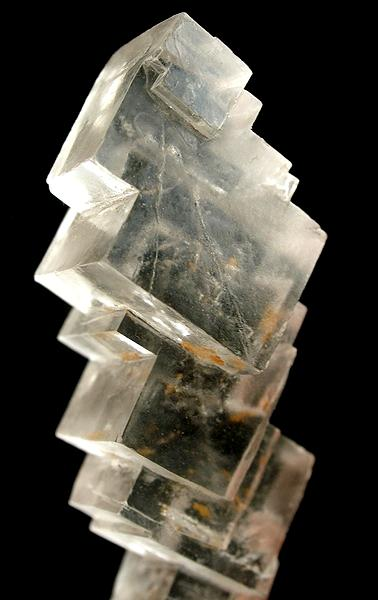
\includegraphics[height=4.6cm]{images/book1/halite.jpg}

{\small Halite, natural rock salt. Photo: Robert M.~Lavinsky,
CC BY-SA 3.0.}
\end{minipage}
\end{omfigure}

\section{Ionic solutions conduct}

\begin{notation}[The state symbol (aq)]\label{not:g9:ions:aq}
An \omterm{def:g9:ions:ion}{ion} or a \omterm{def:g7:atoms-and-molecules:molecule}{molecule} dissolved in water is marked (aq), for aqueous:
\ce{Na+(aq)}, \ce{Cl-(aq)}.
\end{notation}

\begin{proposition}[Ionic solutions conduct electricity]\label{prop:g9:ions:conduct}
When an \omterm{def:g9:ions:ionic-compound}{ionic compound} \omterm{def:g2:mixing-and-dissolving:dissolve}{dissolves} in water, its \omterm{def:g9:ions:ion}{ions} separate and move
freely in the solution: salt water contains \ce{Na+(aq)} and
\ce{Cl-(aq)}. Moving \omterm{def:g9:ions:ion}{ions} carry electric charge, so an ionic solution
conducts electricity. A solution of sugar, whose \omterm{def:g7:atoms-and-molecules:molecule}{molecules} carry no
charge, does not; nor does very pure water.
\end{proposition}

\begin{inthelab}[Which liquids conduct?]
Two metal plates, a low-voltage battery and a small bulb are joined in a
circuit by the teacher; the plates are dipped in turn into distilled
water, sugar water, salt water and a copper sulfate solution, and rinsed
between each. The bulb lights only with the two ionic solutions.
\end{inthelab}

\begin{omfigure}
\begin{tikzpicture}[font=\small, scale=1.1]
  \foreach \xs/\lit/\lab in {0/1/{salt water: the bulb lights}, 5.2/0/{sugar water: it stays dark}} {
    \begin{scope}[xshift=\xs cm]
      \pic[transform shape] at (2,0) {beaker={0.7}{omWater!80}};
      \fill[black!45] (1.6,0.25) rectangle (1.7,2.6);
      \fill[black!45] (2.3,0.25) rectangle (2.4,2.6);
      \ifnum\lit=1 \fill[yellow!70, opacity=0.8] (3.4,3.0) circle (0.42);\fi
      \draw (1.65,2.6) -- (1.65,3.6) to[battery1] (3.4,3.6) -- (3.4,3.4)
        to[lamp] (3.4,2.6) -- (2.35,2.6);
      \node[anchor=north, align=center] at (2,-0.15) {\lab};
    \end{scope}
  }
\end{tikzpicture}

{\small The conductivity test: with salt water, \omterm{def:g9:ions:ion}{ions} carry the current
and the bulb lights; sugar water contains no \omterm{def:g9:ions:ion}{ions} and the bulb stays
dark.}
\end{omfigure}

\section{Precipitation tests for ions}

\begin{definition}[Precipitate]\label{def:g9:ions:precipitate}
When two solutions are mixed, a \omterm{def:g9:ions:ion}{cation} of one and an \omterm{def:g9:ions:ion}{anion} of the other
may form an \omterm{def:g9:ions:ionic-compound}{ionic compound} that does not \omterm{def:g2:mixing-and-dissolving:dissolve}{dissolve}. It appears as a fine
solid that clouds the liquid and settles: a
\emph{precipitate}\index{precipitate}. The reaction is a
\emph{precipitation}\index{precipitation}.
\end{definition}

\begin{proposition}[Tests for common ions]\label{prop:g9:ions:tests}
A few drops of a \omterm{def:g7:identifying-substances:characteristic-test}{reagent} solution identify an \omterm{def:g9:ions:ion}{ion} by the colour of the
\omterm{def:g9:ions:precipitate}{precipitate} it forms:
\begin{center}
\small
\begin{tabular}{llll}
\hline
\omterm{def:g9:ions:ion}{ion} looked for & \omterm{def:g7:identifying-substances:characteristic-test}{reagent} & \omterm{def:g9:ions:precipitate}{precipitate} & colour \\
\hline
copper(II) \ce{Cu^{2+}} & sodium hydroxide & \ce{Cu(OH)2} & blue \\
iron(II) \ce{Fe^{2+}} & sodium hydroxide & \ce{Fe(OH)2} & green \\
iron(III) \ce{Fe^{3+}} & sodium hydroxide & \ce{Fe(OH)3} & orange-brown \\
zinc \ce{Zn^{2+}} & sodium hydroxide & \ce{Zn(OH)2} & white \\
aluminium \ce{Al^{3+}} & sodium hydroxide & \ce{Al(OH)3} & white \\
chloride \ce{Cl-} & silver nitrate & \ce{AgCl} & white, darkens in light \\
\hline
\end{tabular}
\end{center}
\end{proposition}

\begin{example}[Writing a precipitation]\label{ex:g9:ions:equation}
Only the \omterm{def:g9:ions:ion}{ions} that form the solid are written; the others stay dissolved
and take no part:
\[
  \ce{Cu^{2+}(aq) + 2OH-(aq) -> Cu(OH)2(s)}, \qquad
  \ce{Ag+(aq) + Cl-(aq) -> AgCl(s)}.
\]
\end{example}

\begin{omfigure}
\begin{tikzpicture}[font=\small, scale=0.95]
  \foreach \k/\pc/\lab in {0/blue!60/{\ce{Cu^{2+}}: blue}, 1/green!45!black!70/{\ce{Fe^{2+}}: green},
      2/orange!70!brown/{\ce{Fe^{3+}}: orange-\\brown}, 3/white!85!black/{\ce{Zn^{2+}}: white},
      4/white!85!black/{\ce{Al^{3+}}: white}, 5/white!80!black/{\ce{Cl-}: white}} {
    \pic[transform shape] at (\k*2.3,0) {testtube={0.5}{omWater!60}};
    \pic[transform shape] at (\k*2.3,0) {testtube={0.14}{\pc}};
    \node[anchor=north, align=center, font=\footnotesize, text width=2cm] at (\k*2.3,-0.15) {\lab};
  }
\end{tikzpicture}

{\small \omterm{def:g9:ions:precipitate}{Precipitates} formed with sodium hydroxide (first five tubes) and
with silver nitrate (last tube).}
\end{omfigure}

\begin{safety}{\ghs[0.82cm]{GHS05}\ghs[0.82cm]{GHS07}}
% ledger: ghs:NaOH, ghs:AgNO3
Sodium hydroxide: causes severe skin burns and eye damage, and may be
corrosive to metals (GHS05); irritating to skin and eyes in dilute form
(GHS07). Silver nitrate, the chloride
\omterm{def:g7:identifying-substances:characteristic-test}{reagent}, is an oxidiser, corrosive and very toxic to aquatic life.
Goggles, gloves; \omterm{def:g7:identifying-substances:characteristic-test}{reagents} dispensed by drops by the teacher.
\end{safety}

\begin{method}[Testing for an ion]\label{met:g9:ions:test}
\begin{enumerate}
  \item Pour a little of the solution to be tested into a test tube.
  \item Add the \omterm{def:g7:identifying-substances:characteristic-test}{reagent} drop by drop.
  \item Note the colour of any \omterm{def:g9:ions:precipitate}{precipitate} and compare with the table.
  \item Conclude, and remember that a test identifies an \omterm{def:g9:ions:ion}{ion}, not a
        compound: the iron(III) chloride solution gives both the
        \ce{Fe^{3+}} test and the \ce{Cl-} test.
\end{enumerate}
\end{method}

\section{Exercises}

\begin{exercise}[$\star$]\label{exo:g9:ions:1}
What is an \omterm{def:g9:ions:ion}{ion}? What is the difference between a \omterm{def:g9:ions:ion}{cation} and an \omterm{def:g9:ions:ion}{anion}?
\end{exercise}

\begin{exercise}[$\star$]\label{exo:g9:ions:2}
A magnesium \omterm{def:g7:atoms-and-molecules:atom}{atom} (12 \omterm{def:g9:inside-the-atom:proton}{protons}) loses two \omterm{def:g9:inside-the-atom:nucleus}{electrons}. Write the formula of
the \omterm{def:g9:ions:ion}{ion} formed, and give its numbers of \omterm{def:g9:inside-the-atom:proton}{protons} and \omterm{def:g9:inside-the-atom:nucleus}{electrons}.
\end{exercise}

\begin{exercise}[$\star$]\label{exo:g9:ions:3}
Write the formulas of potassium chloride, magnesium chloride and
calcium oxide (oxide \omterm{def:g9:ions:ion}{ion}: \ce{O^{2-}}).
\end{exercise}

\begin{exercise}[$\star$]\label{exo:g9:ions:4}
Why does salt water conduct electricity while sugar water does not?
\end{exercise}

\begin{exercise}[$\star\star$]\label{exo:g9:ions:5}
Write the formulas of copper(II) sulfate, aluminium chloride and sodium
carbonate.
\end{exercise}

\begin{exercise}[$\star\star$]\label{exo:g9:ions:6}
Sodium hydroxide added to a solution gives an orange-brown \omterm{def:g9:ions:precipitate}{precipitate}.
Which \omterm{def:g9:ions:ion}{ion} does the solution contain? Write the equation of the
\omterm{def:g9:ions:precipitate}{precipitation}.
\end{exercise}

\begin{exercise}[$\star\star$]\label{exo:g9:ions:7}
How many \omterm{def:g9:inside-the-atom:nucleus}{electrons} does the sulfate \omterm{def:g9:ions:ion}{ion} \ce{SO4^{2-}} carry in excess of
its \omterm{def:g9:inside-the-atom:proton}{protons}? The nitrate \omterm{def:g9:ions:ion}{ion} \ce{NO3-}?
\end{exercise}

\begin{exercise}[$\star\star$]\label{exo:g9:ions:8}
A solution gives a white \omterm{def:g9:ions:precipitate}{precipitate} with silver nitrate and a blue one
with sodium hydroxide. Name the dissolved \omterm{def:g9:ions:ionic-compound}{ionic compound} and write its
formula.
\end{exercise}

\begin{exercise}[$\star\star$]\label{exo:g9:ions:9}
Look at the figure of the salt crystal layer. How many neighbours of
opposite charge does an \omterm{def:g9:ions:ion}{ion} in the middle of the layer have in this
layer?
\end{exercise}

\begin{exercise}[$\star\star$]\label{exo:g9:ions:10}
Write the equation of the \omterm{def:g9:ions:precipitate}{precipitation} of iron(II) hydroxide from
\ce{Fe^{2+}} and \ce{OH-} \omterm{def:g9:ions:ion}{ions}.
\end{exercise}

\begin{exercise}[$\star\star\star$]\label{exo:g9:ions:11}
A white powder may be zinc chloride or sodium chloride. Dissolved in
water, it gives a white \omterm{def:g9:ions:precipitate}{precipitate} with sodium hydroxide. Which is it?
Write the equation.
\end{exercise}

\begin{exercise}[$\star\star\star$]\label{exo:g9:ions:12}
In a crystal of calcium chloride, how many chloride \omterm{def:g9:ions:ion}{ions} are there for
1000 calcium \omterm{def:g9:ions:ion}{ions}? Check that the crystal is neutral.
\end{exercise}

\section{Problem: The Rusty Well}

\begin{problem}[{Weekend problem --- orange stains in a farmhouse sink,
two tests, and the number of iron ions in a litre of well water}]
\label{pb:g9:ions:1}
The water of a farmhouse well leaves orange stains in the sink. A
laboratory receives a sample. Freshly drawn, the water is clear; with
sodium hydroxide it gives a green \omterm{def:g9:ions:precipitate}{precipitate}, which turns orange-brown
within an hour at the surface, where it meets the \omterm{def:g4:air-a-mixture-of-gases:air}{air}. The laboratory
measures \qty{0.30}{mg} of iron, in the form of iron \omterm{def:g9:ions:ion}{ions}, per litre.
Take the mass of a \omterm{def:g9:inside-the-atom:proton}{nucleon} as \qty{1.67e-27}{kg}, and 56 \omterm{def:g9:inside-the-atom:proton}{nucleons} for an
iron \omterm{def:g7:atoms-and-molecules:atom}{atom}.

\medskip
\noindent\textbf{Part I --- The tests.}
\begin{enumerate}
  \item Which \omterm{def:g9:ions:ion}{ion} does the green \omterm{def:g9:ions:precipitate}{precipitate} show? Give the formula of
        the \omterm{def:g9:ions:precipitate}{precipitate}.
  \item Which \omterm{def:g9:ions:ion}{ion} does the orange-brown \omterm{def:g9:ions:precipitate}{precipitate} show? Give its
        formula.
  \item An iron(II) \omterm{def:g9:ions:ion}{ion} and an iron(III) \omterm{def:g9:ions:ion}{ion} differ by one \omterm{def:g9:inside-the-atom:nucleus}{electron}.
        Which has more \omterm{def:g9:inside-the-atom:nucleus}{electrons}? How many \omterm{def:g9:inside-the-atom:nucleus}{electrons} does each have
        (iron: $Z = 26$)?
  \item Write the equation of the \omterm{def:g9:ions:precipitate}{precipitation} of iron(III) hydroxide.
\end{enumerate}

\medskip
\noindent\textbf{Part II --- The stains.}
\begin{enumerate}[resume]
  \item In the sink, the clear water slowly turns cloudy and orange. Which
        \omterm{def:g9:ions:ion}{ion} does the water hold when it comes out of the well, and which
        does it end up holding?
  \item Write the formula of the \omterm{def:g9:ions:ionic-compound}{ionic compound} formed by iron(III) \omterm{def:g9:ions:ion}{ions}
        and hydroxide \omterm{def:g9:ions:ion}{ions}, and check that it is neutral.
  \item Can the iron of the water be removed by \omterm{def:g3:separating-mixtures:filter}{filtering} the water as it
        comes out of the well? After it has turned orange? Explain.
  \item Is a water containing iron \omterm{def:g9:ions:ion}{ions} a \omterm{def:g6:pure-substances-and-mixtures:pure-substance}{pure substance}? A \omterm{def:g6:pure-substances-and-mixtures:homogeneous}{homogeneous
        mixture}?
\end{enumerate}

\medskip
\noindent\textbf{Part III --- Counting the \omterm{def:g9:ions:ion}{ions}.}
\begin{enumerate}[resume]
  \item Compute the mass of an iron \omterm{def:g7:atoms-and-molecules:atom}{atom}, in kilograms.
  \item Convert \qty{0.30}{mg} into kilograms.
  \item Why may the mass of an iron \omterm{def:g9:ions:ion}{ion} be taken equal to that of an iron
        \omterm{def:g7:atoms-and-molecules:atom}{atom}?
  \item Compute the number of iron \omterm{def:g9:ions:ion}{ions} in a litre of the well water.
\end{enumerate}
\end{problem}
